%\usepackage[a4paper,top=0.2cm,bottom=0.1cm,left=1.5cm,right=1cm,marginparwidth=0.75cm]{geometry}


\documentclass[a4paper,12pt]{article} % добавить leqno в [] для нумерации слева
\usepackage[left=1.5cm,right=1.5cm,top=2cm,bottom=2cm]{geometry}
%%% Работа с русским языком
\usepackage{cmap}					% поиск в PDF
\usepackage{mathtext} 				% русские буквы в формулах
\usepackage[T2A]{fontenc}			% кодировка
\usepackage[utf8]{inputenc}			% кодировка исходного текста
\usepackage[english,russian]{babel}	% локализация и переносы
\usepackage{subfig}
\usepackage{float}

%%% Работа с русским языком
\usepackage{cmap}                           % поиск в PDF
\usepackage{mathtext} 			 	       % русские буквы в формулах
\usepackage[T2A]{fontenc}               % кодировка
\usepackage[utf8]{inputenc}              % кодировка исходного текста
\usepackage[section]{placeins}
\usepackage[english,russian]{babel}  % локализация и переносы

\usepackage{graphicx}
\graphicspath{{noiseimages/}}
\usepackage{wrapfig}
\usepackage{tabularx}
\usepackage{hyphenat}
\usepackage{hyperref}
\usepackage{gensymb}
\usepackage[rgb]{xcolor}
\hypersetup{
colorlinks=true,urlcolor=blue
}


%%% Дополнительная работа с математикой
\usepackage{amsmath,amsfonts,amssymb,amsthm,mathtools} % AMS
\usepackage{icomma} % "Умная" запятая: $0,2$ --- число, $0, 2$ --- перечисление

%% Номера формул
%\mathtoolsset{showonlyrefs=true} % Показывать номера только у тех формул, на которые есть \eqref{} в тексте.

%% Шрифты
\usepackage{euscript}	 % Шрифт Евклид
\usepackage{mathrsfs} % Красивый матшрифт

%% Свои команды
\DeclareMathOperator{\sgn}{\mathop{sgn}}

%% Перенос знаков в формулах (по Львовскому)
\newcommand*{\hm}[1]{#1\nobreak\discretionary{}
{\hbox{$\mathsurround=0pt #1$}}{}}




\date{\today}

\begin{document}

\begin{titlepage}
\centering    

\begin{figure}[t]
\centering

\includegraphics[width=100mm]{frtk-label 2.jpg}
\label{frkt-label.jpg}
\end{figure}




\author{Сурженко Эдуард Б01-304}
\title{3.2.6 Изучение гальванометра}
\date{}
%\begin{document}
\maketitle
\vfill
% Bottom of the page
	Долгопрудный, 2024 г.
\thispagestyle{empty}
\end{titlepage}
\textbf{Цель работы:} 
Изучение работы высокочувствительного зеркального гальванометра магнитоэлектпической системы в режимах измерения постоянного тока и электрического заряда.

\textbf{В работе используются:}
Зеркальный гальванометр с осветителем и шкалой, источник постоянного напряжения, делитель напряжения, магазин сопротивлений, эталонный конденсатор, вольтметр, переключатель, ключи, линейка.

\section{Определение динамической постоянной гальванометра}
\subsection{Установка}
\begin{figure}[h!]
    \centering
    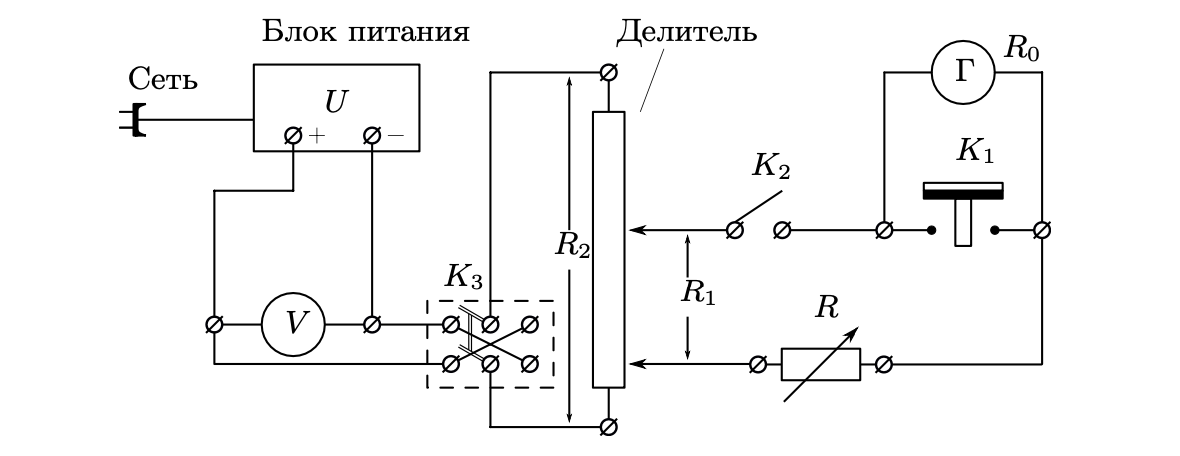
\includegraphics[width=0.8\linewidth]{Снимок экрана 2024-11-15 в 21.42.32.png}
    \caption{Схема установки для работы гальванометра в стационарном режиме}
    \label{sheme_1}
\end{figure}
\begin{centering}
\textit{Вольтметр V измеряет постоянное напряжение U. Ключ $K_3$ меняeт направление тока через гальванометр Г. Делитель напряжения позволяет менять величину тока. Ключ $K_2$ служит для включения гальванометра. Кнопка $K_1$ успокаивает гальванометр. Магазин сопротивлений R позволяет менять режим работы гальванометра.}
\end{centering}
\newline
\newline
Ключ $K_1$ служит для успокоения гальваномета посредством его отключения от источника тока, что помогает избежать влияния внешних электрических шумов и колебаний на его показания. Это важно при измерении малых токов, где каждое колебание может привести к значительным ошибкам. 
\newpage
\subsection{Гальванометр}
\begin{figure}[h!]
    \centering
    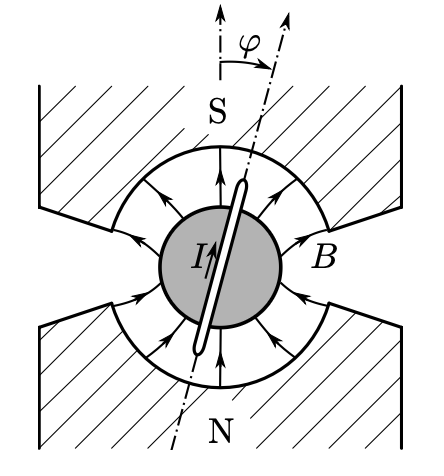
\includegraphics[width=0.3\linewidth]{Galvanometr.png}
    \caption{Рамка с током в магнитном поле}
    \label{fig:enter-label}
\end{figure}
\begin{raggedright}
Главной частью высокочувствительного гальванометра магнитоэлектрической системы является подвешенная на вертикальной нити рамка, помещённая в поле постоянного магнита (рис. 2). Вырез цилиндрической формы в полюсах магнита и ферромагнитный цилиндр на оси системы делают поле в зазоре радиальным. Скреплённое с рамкой зеркальце служит для измерения угла поворота рамки. Магнит и подвижная система заключены в защитный кожух.
\end{raggedright}
\begin{centering}
Запишем основное уравнение колебаний рамки:
\end{centering}
\begin{equation}\label{main}
\ddot{\phi} + 2\gamma\dot{\phi }+ \omega_0^2\phi = K I
\end{equation}
где введены обозначения: $ 2\gamma = \dfrac{(BSN)^2}{JR_\Sigma} $, $ \omega_0^2 = \dfrac{D}{J}, K = \dfrac{BSN}{J} $. Эти величины выражены через параметры установки: $ B $ --- магнитное поле, в которое помещена рамка, $ I  = \dfrac{\mathcal{E}}{R_\Sigma}$ --- ток, текущий через рамку, $ R_\Sigma $ --- сопротивление рамки и цепи, $ N $ --- число витков рамки, $ S $ --- площадь витка рамки, $ J $ --- момент инерции системы, $ D $ --- модуль кручения нити.
	


\subsection{Теоретическая выкладка}
При $R_1$ $\ll$ R, $R_0$, $R_2$ сила тока, протекающего через гальванометр, может быть вычислена как
\begin{equation}
I = \frac{R_1}{R_2} \frac{U_0}{R+R_0}    
\end{equation}


где $U_0$ - показания вольтметра, $R_1/R_2$ - положение делителя, R - сопротивление магазина, $R_0$ - внутреннее сопротивление гальванометра.
Угол отклонения рамки от положения равновесия измеряется с помощью осветителя, зеркальца, укреплённого на рамке, и шкалы, на которую отбрасывается луч света от зеркальца. Координата x святового пятна на шкале связана с углом $\varphi$ отклонения рамки формулой:
\begin{equation}
x = a \arctan{2\varphi}
\end{equation}
где a - расстояние от шкалы до зеркальца. При малых углах можно считать, что $\varphi$ = x/2a.
\\
Динамическая постоянная:
\begin{equation}
C_I = \frac{I}{\varphi} = \frac{2aI}{x} \\ \\ \left[ \frac{A}{\text{мм}/\text{м}} \right]
\end{equation}
\subsection{A. Обработка результатов}
\[
R1/R2 = 1/1000; \ \ R_0 = 610 \pm 5\text{ Ом}; \ \ R_2=10 \pm 0,1 \text{ кОМ}; \ \ R = 50 \pm 0,5 \text{ кОм}; \ \ U_0 = 1,18 \text{ В}; \ \ a = 1,35 \text{ м}
\]
Измерив токи I, построим график зависимости I(x) для различных значений сопротивлений магазина R:
\begin{figure}[h!]
    \centering
    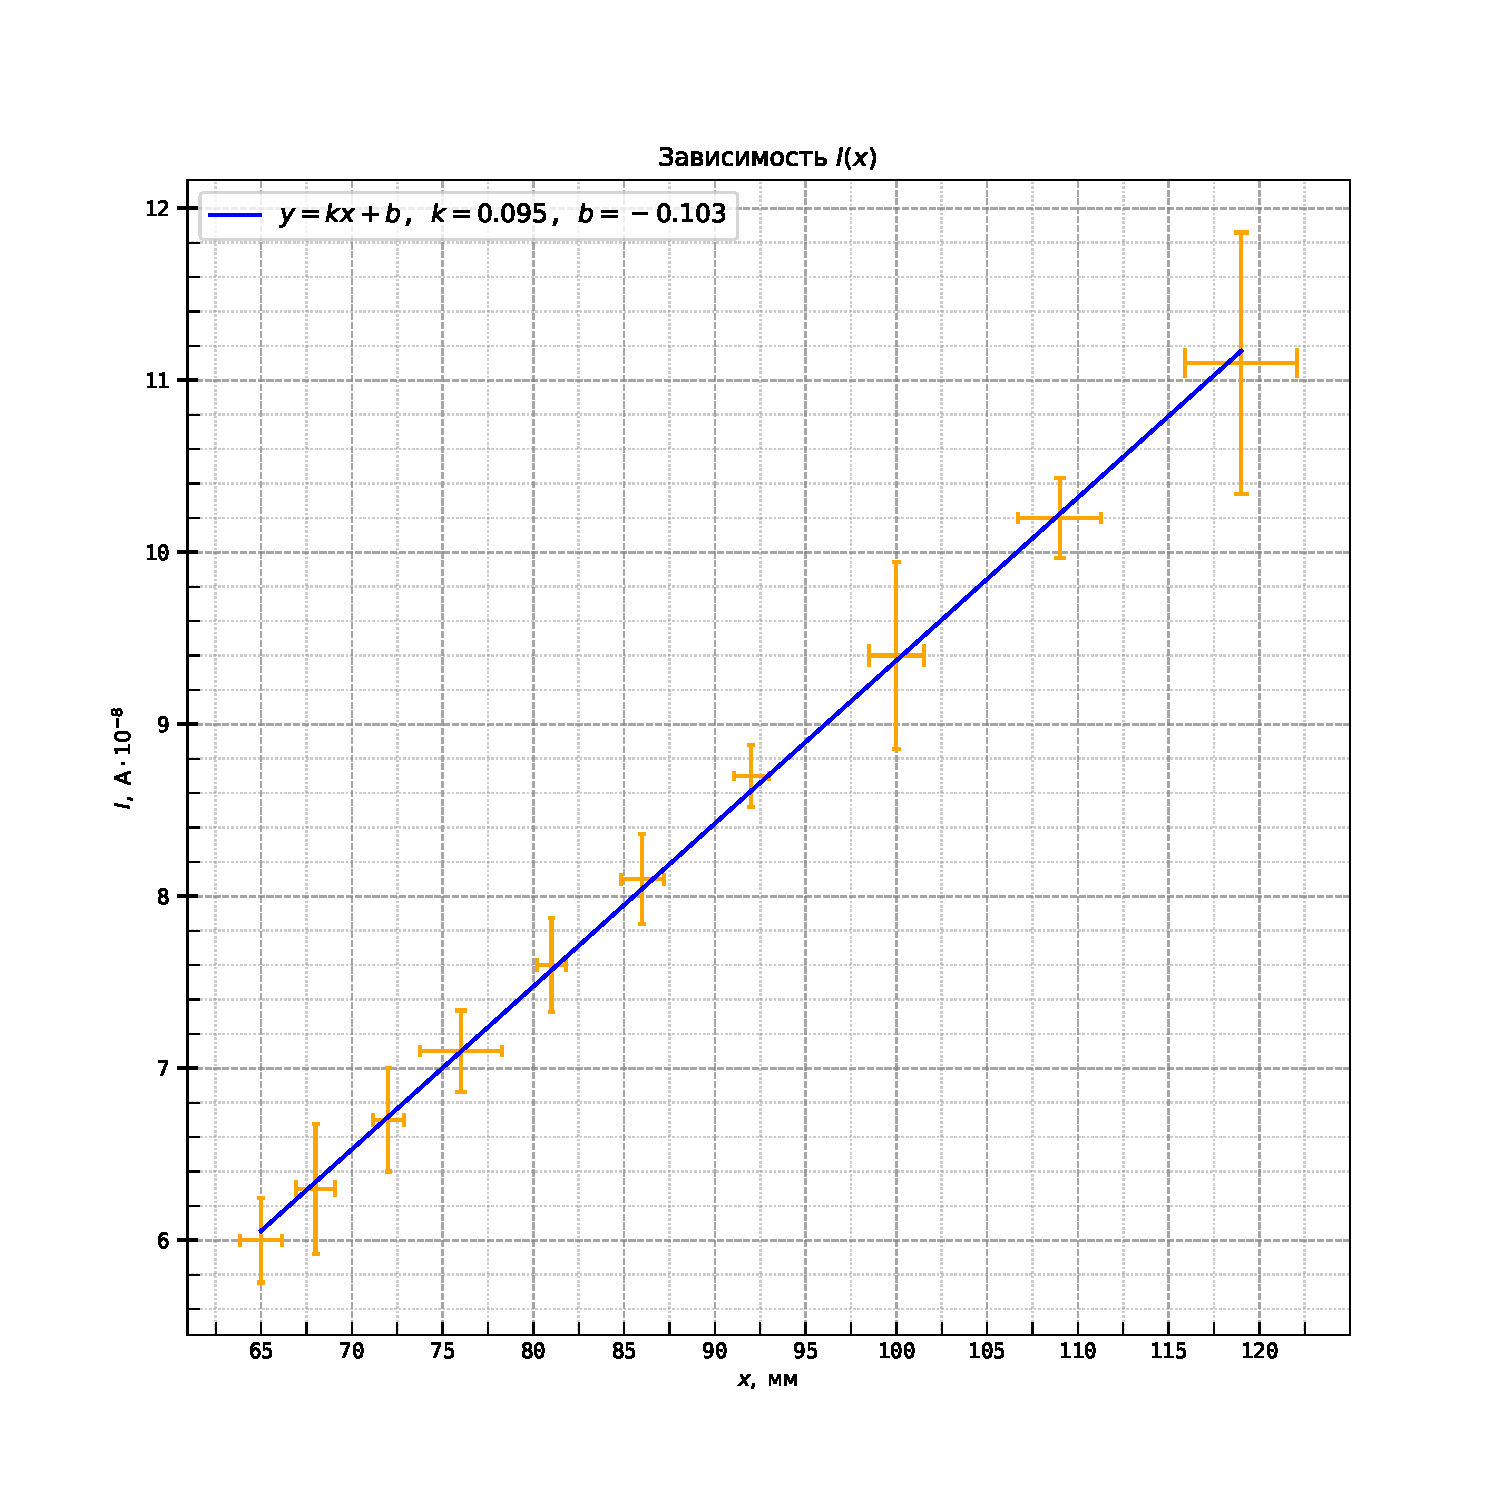
\includegraphics[width=0.8\linewidth]{graphic.pdf}
    \caption{График зависимости I(x)}
    \label{fig:enter-label}
\end{figure}
\\
Тангенс угла наклона $tg\alpha = (0,095 \pm 0,007) \cdot 10^{-8} \frac{\text{А}}{\text{мм}}$.
\\
\[
\frac{\sigma_{C_I}}{C_I} = \sqrt{\left(\frac{\sigma_a}{a}\right)^2+\left(\frac{\sigma_{tg\alpha}}{tg\alpha}\right)^2} \approx 0,07
\]
Подставляя значения в формулу (4), находим значения по формуле -- $C_I = 2a\text{ tg}\alpha$
Динамическая постоянная:
\[
C_I = 2,6 \pm 0,2 \ \ \left[ \frac{\text{нА}}{\text{мм}/\text{м}} \right]
\]
Чувствительность к току:
\[
S_I = C_I^{-1} = 0,38 \pm 0,03 \ \ \left[ \frac{\text{мм}/\text{м}}{\text{нА}} \right]
\]

\section{Определение критического сопротивления гальванометра}
\subsection{Теоретическое выкладка}
Критическим сопротивлением баллистического гальванометра называется сопротивление его электрической цепи $R_\text{кр}$, при котором после начального толчка подвижная система почти экспоненциально возвращается к нулю, подчиняясь уравнению:
\begin{equation}
R_\text{кр} = R_{\Sigma\text{кр}} - R_0 = \frac{(BSN)^2}{2 \sqrt{DJ}} - R_0   
\end{equation}
На практике критический режим, требующий строгого выполнения условия $\gamma = \omega_0$, не может быть точно реализован и имеет значение как пограничный между режимом затухающих колебаний ($\gamma < \omega_0$) и режимом апериодического затухания ($\gamma > \omega_0$)
\\
В качестве характеристики процесса затухания колебаний рамки гальванометра воспользуемся логарифмическим декрементом затухания:
\begin{equation}
    \Theta = \gamma T_1 = ln\frac{x_n}{x_{n+1}}
\end{equation}
где $x_n$ и $x_{n+1}$ - два последовательных отклонения колеблющейся величины в одну сторону. Измеряя зависимость $\Theta(R)$ логарифмического декремента затухания от сопротивления внешней цепи R, можно найти 
критическое сопротивление $R_\text{кр}$
\\
Используя,
\[
\Theta = \gamma T_1 = \frac{(BSN)^2}{2 J R_\Sigma} \cdot 2\pi \left[ \frac{D}{J} - \frac{(BSN)^4}{(2JR_\Sigma)^2}\right]^{-1/2}
\]
Приведём к виду:
\[
\left(\frac{2\pi}{\Theta}\right)^2+1 = \frac{(2JR_\Sigma)^2}{(BSN)^4} \cdot \frac{D}{J}
\]
подставим в формулу (5) и получим:
\begin{equation}
    R_\text{кр} = \frac{R+R_0}{\sqrt{\left(\frac{2 \pi}{\Theta}\right)^2+1}} - R_0
\end{equation}
или
\begin{equation}
    \sqrt{\frac{4 \pi^2}{\Theta^2} + 1} = \frac{R+R_0}{R_\text{кр}+R_0}
\end{equation}

\subsection{Б. Обработка результатов}
Установим сопротивление, при котором зайчик отклонится почти на всю шкалу:
\[
R = 5,00 \pm 0,05 \text{ кОм}
\]
Зайчик при этом отклонился на $x_1 = 18,6 \pm 0,2 \text{ см}$ и $x_2 = 15,3 \pm 0,2 \text{ см}$
\\
\newline
Рассчитаем логарифмический декремент затухания $\Theta_0$ по формуле (6):
\[
\Theta_0 = 0.196 \pm 0,017
\]
Период $T_0$ свободных колебаний рамки:
\[
T_0 = 3.71 \pm 0,07 \text{ c}
\]
Рассчитаем декремент затухания $\Theta$ при:
\[
R_1/R_2 = 1/300 - \text{положение делителя}
\]
\[
R_\text{кр} = 7,800 \pm 0,078\text{ кОм} - \text{критическое споротивление}
\]
\[
R = 3 \cdot R_\text{кр} = 23,40 \pm 0,23\text{ кОм}
\]
из формулы (6) он получается равным:
\[
\Theta = 1,65 \pm 0,01
\]
Теперь рассчитаем $\Theta$ по формуле (6) для других значений R, увеличивая его c 3$R_\text{кр}$ до $10R_\text{кр}$ и подставим в формулу (7) (см. Таблица 1 в приложении).
\\
Найдём $R_\text{кр}$, посчитав истинное среднее с помощью распределения Стьюдента:
\begin{equation}
R_\text{кр} = \left<R_\text{кр}\right> \pm A \frac{\sigma_R}{\sqrt{N}}
\end{equation}
где A = 2,015 - коэффициент Стьюдента, $\left<R_\text{кр}\right>$ = 5,86\text{ кОм} - среднее арифмитическое $R_\text{кр}$;
\\$\sigma_R$ = 0,13 кОм - среднеквадратичное отклонение. N = 15. Получаем ответ:
\[
R_\text{кр} = 5,86 \pm 0,06 \text{ кОм}
\]

\newpage

\section{Определение баллистической постоянной и критического сопротивления гальванометра, работающего в баллистическом режиме}
\subsection{Схема}
\begin{figure}[h!]
    \centering
    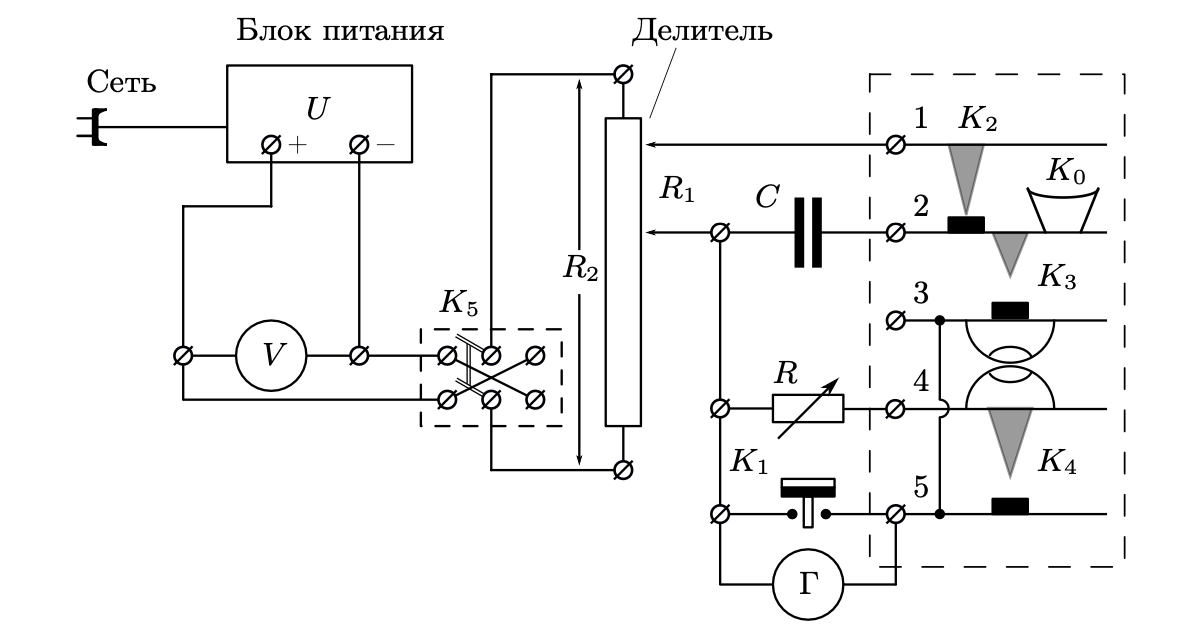
\includegraphics[width=0.8\linewidth]{Снимок экрана 2024-11-16 в 02.47.25.png}
    \caption{Схема установки для определения баллистического постоянной}
    \label{sheme-3}
\end{figure}
Система ключей устрона так, что нормально ключ $K_2$ замкнут, а ключи $K_3$ и $K_4$ разомкнуты. При нажатии на кнопку $K_0$ сначала размыкается ключ $K_2$, затем $K_3$ и через некоторые время - $K_4$. При нормальном положении кнопки $K_0$ конденсатор $C$ заряжается до напряжение $U_C$ и получается заряд q:
\[
U_C = \frac{R_1}{R_2} U_0 \ \ \ \ q = CU_C = \frac{R_1}{R_2}U_0C
\]
При нажатии на ключ $K_0$ конденсатор отключается от источника постоянного напряжения (размыкается ключ $K_2$) и подключается к гальванометру (замыкается ключ $K_3$).
\subsection{Теоретическая выкладка}
Ёмкость конденсатора выбрана так, что к моменту замыкания ключа $K_4$ весь заряд успевает пройти через гальванометр, и рамка получает начальную скорость $\dot\varphi(\tau) = Kq$. При этом можно считать, что отклонение рамки, происходящее за время, протекающее между замыканием ключей $K_3$ и $K_4$, равно нулю. При замыкании ключа $K_4$ гальванометр шунтируется внешним сопротивлением R, и в зависимости от величины этого споротивления движение рамки описывается одним из следующих уравнений:
\\
При $\gamma < \omega_0$ (колебательный режим):
\begin{equation}
\varphi(t) = \frac{\dot\varphi_0}{\omega_1}e^{-\gamma t}\sin{\omega_1t},
\  \  \  \  \  \  \
\omega_1 = \sqrt{\omega_0^2 - \gamma^2}
\end{equation}
Когда $\gamma \ll \omega_0$ (малое затухание), $\omega_1 \approx \omega_0$, движение рамки близко к синусоидальному:
\begin{equation}
\varphi(t) = \frac{\dot\varphi_0}{\omega_0}\sin{\omega_0t}
\end{equation}
При $\gamma = \omega$ (критический режим):
\begin{equation}
\varphi(t) = \dot\varphi_0te^{-\gamma t}
\end{equation}
При $\gamma > \omega_0$ (случай переуспокоенного гальванометра):
\begin{equation}
\varphi(t) = \frac{\dot\varphi_0}{\alpha}e^{-\gamma t}sh{\alpha t} 
\  \  \  \  \  \  \
\alpha = \sqrt{\gamma^2 - \omega_0^2}
\end{equation}
Первый отброс зайчика $\varphi_{max}$ после нажатия на кнопку $K_0$ зависит от сопротивления внешней цепи, подключённой к гальванометру. Для определения $R_\text{кр}$ использует то обстоятельство, что в кртичическом режиме максимальное отклонение зайчика в \textit{e} раз меньше, чем у гальванометра без затухания
\begin{equation}
\dot{\varphi}\big|_{0}^{\tau} + 2\gamma \varphi\big|_{0}^{\tau} + \omega_0^2 \int_{0}^{\tau} \varphi \, dt = Kq,
\end{equation}
\\
\begin{equation}
\dot\varphi(\tau) = Kq
\end{equation}
Наблюдать колебания рамки при полном отуствии затухания невозможно. Величину максимального отклонения рамки гальванометра без затухания $\varphi^{\text{св}}_{max}$ можно, однако, рассчитывать, если при разомкнутой цепи измерить реальное максимальное отклонение рамки $\varphi_0$ и логарифмический декремент затухания $\Theta_0$ (При R = $\infty$ величина $\Theta_0$ определяется только внутренним трением в рамке). Из уравнений (5) и (9) при $\gamma \ll \omega_0$ вытекают равенства:
\begin{equation}
    \varphi_0 = \varphi(T_1/4) = \varphi^{\text{св}}_{max}e^{-\Theta_0/4},
\end{equation}
так что максимальное отклонение рамки гальванометра без затухания
\begin{equation}
    \varphi^{\text{св}}_{max} = \varphi_0e^{\Theta_0/4} \approx \varphi_0 \left(1 + \frac{\Theta}{4}\right)
\end{equation}
Баллистическая постоянная гальванометра $C^{\text{кр}}_q \ \ \left[\frac{\text{Кл}}{\text{мм/м}} \right]$ определяется при критическом сопротивлении (R = $R_\text{кр}$):
\begin{equation}
    C^{\text{кр}}_q = \frac{q}{\varphi^{\text{кр}}_{max}} = 2a \frac{R_1}{R_2}\frac{CU_0}{x^{\text{кр}}_{max}}
\end{equation}
где $x^{\text{кр}}_{max}$ - величина первого отброса в критическом режиме, выраженная в делениях шкалы (мм), а - расстояние от зеркальца до шкалы (м), $CU_0$ - заряд (Кл).
\newpage
\subsection{В. Обработка результатов}
\[
C = 2 \text{ мкФ}; \ \ R_1/R_2 = 1/20; \ \ x_{max} = 197 \pm 2 \text{ мм} \ \  (\text{при } \ \ R = \infty); \ \ T = 3,714 \pm 0,148 \text{ с}
\]
Построим график зависисмости отклонения гальванометра от суммарного сопротивления:

\begin{figure}[h!]
    \centering
    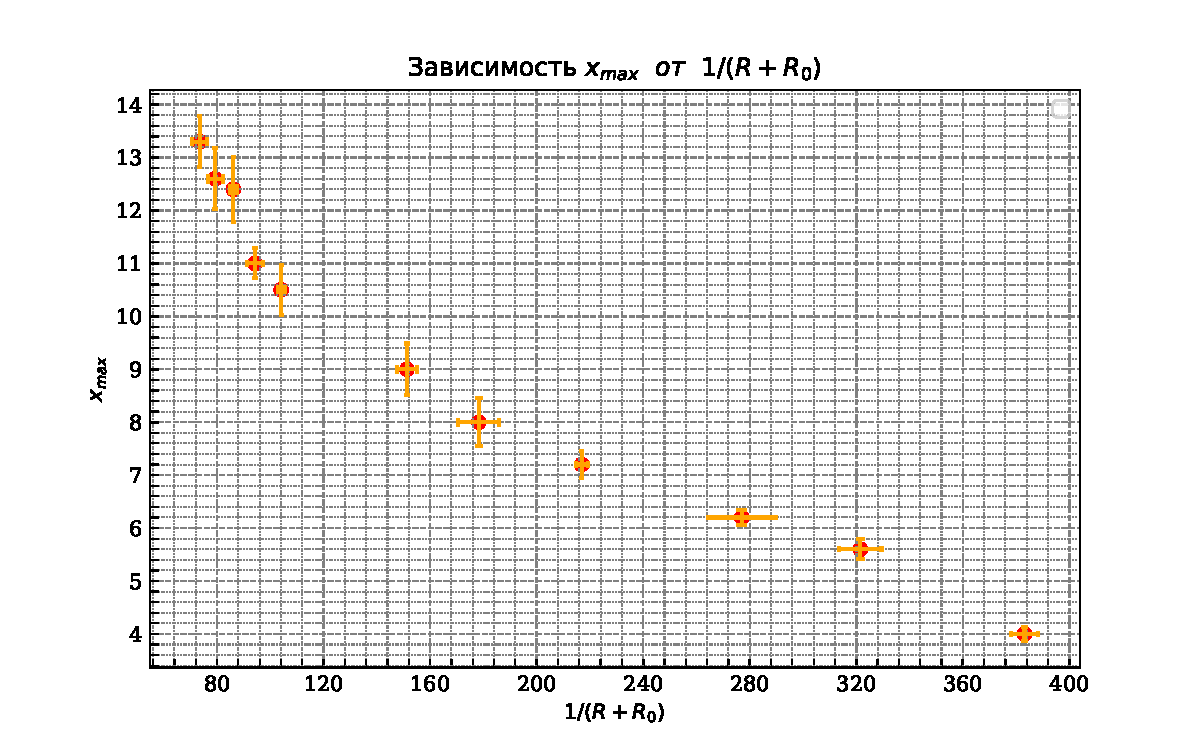
\includegraphics[width=1\linewidth]{graph3_data_2.pdf}
    \label{fig:enter-label}
\end{figure}
Найдём величину $x_1$ = $x_{max} \cdot  e^{\Theta_0/4} $ = 20,68 см. Величина в $\text{e}$ раз меньшая, это $x_e \approx$ 7,60 см. С помощью графика видим, что эта величина соответствует значению $\frac{1}{R+R_0} = (200.072 \pm 14,001)\cdot 10^{-6}\text{ Ом}^{-1}$, получаем:
\[
R   = 4,38 \pm 0,30 \text{ кОм} 
\]
Сравнивая $R_\text{кр} = 4,38 \text{ кОм}$  для баллистического режима с $R_\text{кр} = 5 \text{ кОм}$, получившегося подбором и $R_\text{кр} = 5,86 \text{ кОм}$, получившегося путём рассчёта логарифмических декрементов для различных R, приходим к выводу, что они пересекаются с погрешностью в 14\%. Такая большая погрешность может быть связана с неточностью измерений углов поворота рамки.
\\
Теперь найдём баллистическую постоянную по формуле (18):
\[
C_q^{\text{кр}} = 7,24 \text{ Кл}
\]
Посчитаем погрешность по формуле:
\[
\sigma_{C^{\text{кр}}_q} = C^{\text{кр}}_q \sqrt{\left(\frac{\sigma_U}{U_0}\right)^2 + \left(\frac{\sigma_a}{a}\right)^2+\left(\frac{\sigma_{x_e}}{x_e}\right)^2} = 0,03 \cdot 10^{-6} \text{ Кл} 
\]
Получаем:
\[
 C^{\text{кр}}_q = (7,24 \pm 0,03) \cdot 10^{-6} \text{ Кл} = (7,24 \pm 0,03) \cdot 10^{-3} \ \ \frac{\text{Кл}}{\text{мм/м}}
\]
Посчитаем период релаксации и сравним с периодом свободных колебаний:
\[
\tau = R_0 C \approx 4,42 \pm 0,04\text{ мс}
\]
\[
\frac{T}{\tau} \approx (0,84 \pm 0,03) \cdot 10^3 
\]
\section{Вывод}
1. В этой работе мы исследовали работу гальванометра в трех режимах: стационарном, баллистическом и при свободных колебаниях. Мы измерили критическое сопротивление контура $R_\text{кр}$ тремя способами и выявили высокую погрешность измерения в 14\%, что может быть связано с фактором недостаточной точности измерения отклонений 'зеркальца', электрических шумов, невозможности моментально погасить инерцию отклоняющегося гальванометра. 
\\
2. В ходе работы также нашли динамическую постоянную гальванометра: $C_I = 2,6 \pm0,2 \left[\frac{\text{нА}}{\text{мм/м}}\right]$, которая определяет количество электричества, при протекании которого через рамку последняя повернётся на угол, равный 1 радиану. 
\\
Баллистическую постоянную: $C_q^\text{кр} =(7,24 \pm 0,03) \cdot 10^{-3} \left[ \frac{\text{Кл}}{\text{мм/м}}\right]$, которая показывает, какой заряд (в кулонах) протекает через рамку при смещении светового “зайчика” на одно деление шкалы.

\section{Приложение}



%%
\begin{table}[ht]
\centering
\begin{tabular}{|c|c|c|c|}
\hline
$N$ & $R, \ \text{kОм}$ & $\Theta$ & $R_{\text{кр}}, \ \text{kОм}$ \\
\hline
1  & 26,00 $\pm$ 0,26   & 2,83 $\pm$ 0,01  & 3,868 $\pm$ 0,038   \\
2  & 28,60 $\pm$ 0,29   & 2,81 $\pm$ 0,01  & 4,248 $\pm$ 0,043   \\
3  & 31,20 $\pm$ 0,31   & 2,84 $\pm$ 0,01  & 4,782 $\pm$ 0,048   \\
4  & 33,60 $\pm$ 0,34   & 2,81 $\pm$ 0,01  & 5,080 $\pm$ 0,051   \\
5  & 36,40 $\pm$ 0,36   & 2,80 $\pm$ 0,01  & 5,534 $\pm$ 0,055   \\
6  & 39,00 $\pm$ 0,39   & 2,85 $\pm$ 0,01  & 6,134 $\pm$ 0,062   \\
7  & 41,60 $\pm$ 0,42   & 2,82 $\pm$ 0,01  & 6,454 $\pm$ 0,065   \\
8  & 44,20 $\pm$ 0,44   & 2,84 $\pm$ 0,01  & 6,975 $\pm$ 0,071   \\
9  & 46,80 $\pm$ 0,47   & 2,79 $\pm$ 0,01  & 7,179 $\pm$ 0,073   \\
10 & 52,00 $\pm$ 0,52   & 2,72 $\pm$ 0,01  & 7,714 $\pm$ 0,078   \\
11 & 57,20 $\pm$ 0,57   & 2,69 $\pm$ 0,01  & 8,366 $\pm$ 0,085   \\
12 & 62,40 $\pm$ 0,62   & 2,53 $\pm$ 0,01  & 8,159 $\pm$ 0,083   \\
13 & 67,60 $\pm$ 0,68   & 2,05 $\pm$ 0,01  & 5,965 $\pm$ 0,061   \\
14 & 72,80 $\pm$ 0,73   & 1,83 $\pm$ 0,01  & 5,142 $\pm$ 0,052   \\
15 & 78,00 $\pm$ 0,78   & 1,24 $\pm$ 0,01  & 2,341 $\pm$ 0,024   \\
\hline
\end{tabular}
\caption{Таблица значений для разных значений $R$}
\end{table}



%%

\end{document}
